% !TEX TS-program = knitr
\documentclass[handout]{beamer}\usepackage{graphicx, color}
%% maxwidth is the original width if it is less than linewidth
%% otherwise use linewidth (to make sure the graphics do not exceed the margin)
\makeatletter
\def\maxwidth{ %
  \ifdim\Gin@nat@width>\linewidth
    \linewidth
  \else
    \Gin@nat@width
  \fi
}
\makeatother

\definecolor{fgcolor}{rgb}{0.2, 0.2, 0.2}
\newcommand{\hlnumber}[1]{\textcolor[rgb]{0,0,0}{#1}}%
\newcommand{\hlfunctioncall}[1]{\textcolor[rgb]{0.501960784313725,0,0.329411764705882}{\textbf{#1}}}%
\newcommand{\hlstring}[1]{\textcolor[rgb]{0.6,0.6,1}{#1}}%
\newcommand{\hlkeyword}[1]{\textcolor[rgb]{0,0,0}{\textbf{#1}}}%
\newcommand{\hlargument}[1]{\textcolor[rgb]{0.690196078431373,0.250980392156863,0.0196078431372549}{#1}}%
\newcommand{\hlcomment}[1]{\textcolor[rgb]{0.180392156862745,0.6,0.341176470588235}{#1}}%
\newcommand{\hlroxygencomment}[1]{\textcolor[rgb]{0.43921568627451,0.47843137254902,0.701960784313725}{#1}}%
\newcommand{\hlformalargs}[1]{\textcolor[rgb]{0.690196078431373,0.250980392156863,0.0196078431372549}{#1}}%
\newcommand{\hleqformalargs}[1]{\textcolor[rgb]{0.690196078431373,0.250980392156863,0.0196078431372549}{#1}}%
\newcommand{\hlassignement}[1]{\textcolor[rgb]{0,0,0}{\textbf{#1}}}%
\newcommand{\hlpackage}[1]{\textcolor[rgb]{0.588235294117647,0.709803921568627,0.145098039215686}{#1}}%
\newcommand{\hlslot}[1]{\textit{#1}}%
\newcommand{\hlsymbol}[1]{\textcolor[rgb]{0,0,0}{#1}}%
\newcommand{\hlprompt}[1]{\textcolor[rgb]{0.2,0.2,0.2}{#1}}%

\usepackage{framed}
\makeatletter
\newenvironment{kframe}{%
 \def\at@end@of@kframe{}%
 \ifinner\ifhmode%
  \def\at@end@of@kframe{\end{minipage}}%
  \begin{minipage}{\columnwidth}%
 \fi\fi%
 \def\FrameCommand##1{\hskip\@totalleftmargin \hskip-\fboxsep
 \colorbox{shadecolor}{##1}\hskip-\fboxsep
     % There is no \\@totalrightmargin, so:
     \hskip-\linewidth \hskip-\@totalleftmargin \hskip\columnwidth}%
 \MakeFramed {\advance\hsize-\width
   \@totalleftmargin\z@ \linewidth\hsize
   \@setminipage}}%
 {\par\unskip\endMakeFramed%
 \at@end@of@kframe}
\makeatother

\definecolor{shadecolor}{rgb}{.97, .97, .97}
\definecolor{messagecolor}{rgb}{0, 0, 0}
\definecolor{warningcolor}{rgb}{1, 0, 1}
\definecolor{errorcolor}{rgb}{1, 0, 0}
\newenvironment{knitrout}{}{} % an empty environment to be redefined in TeX

\usepackage{alltt}
\newcommand{\answers}{1}

\usetheme{Marburg}
\setbeamertemplate{navigation symbols}{} 
\setbeamertemplate{footline}
{
  \leavevmode%
  \hbox{%
  \begin{beamercolorbox}[wd=.333333\paperwidth,ht=2.25ex,dp=1ex,center]{author in head/foot}%
    \usebeamerfont{author in head/foot}\copyright $\ $ \insertshortauthor%~~\beamer@ifempty{\insertshortinstitute}{}{(\insertshortinstitute)}
  \end{beamercolorbox}%
  \begin{beamercolorbox}[wd=.333333\paperwidth,ht=2.25ex,dp=1ex,center]{title in head/foot}%
    \usebeamerfont{title in head/foot} \insertinstitute
  \end{beamercolorbox}%
  \begin{beamercolorbox}[wd=.333333\paperwidth,ht=2.25ex,dp=1ex,right]{date in head/foot}%
    \usebeamerfont{date in head/foot}\insertshortdate{}\hspace*{2em}
    \insertframenumber{} / \inserttotalframenumber\hspace*{2ex} 
  \end{beamercolorbox}}%
  \vskip0pt%
}

\usepackage{amsmath}
\usepackage{caption}
\usepackage{color}
\usepackage{enumerate}
\usepackage{listings}
\usepackage{hyperref}
\usepackage{mathrsfs}
\usepackage{natbib}
\usepackage{url}

\providecommand{\all}{\ \forall \ }
\providecommand{\bs}{\backslash}
\providecommand{\e}{\varepsilon}
\providecommand{\E}{\ \exists \ }
\providecommand{\lm}[2]{\lim_{#1 \rightarrow #2}}
\providecommand{\m}[1]{\mathbb{#1}}
\providecommand{\nv}{{}^{-1}}
\providecommand{\ov}[1]{\overline{#1}}
\providecommand{\p}{\newpage}
\providecommand{\q}{$\quad$ \newline}
\providecommand{\rt}{\rightarrow}
\providecommand{\Rt}{\Rightarrow}
\providecommand{\vc}[1]{\boldsymbol{#1}}
\providecommand{\wh}[1]{\widehat{#1}}

\hypersetup{colorlinks,linkcolor=,urlcolor=blue}
\numberwithin{equation}{section}

\definecolor{dkgreen}{rgb}{0,0.6,0}
\definecolor{gray}{rgb}{0.5,0.5,0.5}
\definecolor{mauve}{rgb}{0.58,0,0.82}

\lstset{ 
  language=C,                % the language of the code
  basicstyle= \footnotesize,           % the size of the fonts that are used for the code
  numberstyle= \tiny \color{white},  % the style that is used for the line-numbers
  stepnumber=2,                   % the step between two line-numbers. 
  numbersep=5pt,                  % how far the line-numbers are from the code
  backgroundcolor=\color{white},      % choose the background color. You must add \usepackage{color}
  showspaces=false,               % show spaces adding particular underscores
  showstringspaces=false,         % underline spaces within strings
  showtabs=false,                 % show tabs within strings adding particular underscores
  frame=lrb,                   % adds a frame around the code
  rulecolor=\color{black},        % if not set, the frame-color may be changed on line-breaks within not-black text 
  tabsize=2,                      % sets default tabsize to 2 spaces
  captionpos=t,                   % sets the caption-position 
  breaklines=true,                % sets automatic line breaking
  breakatwhitespace=false,        % sets if automatic breaks should only happen at whitespace
  %title=\lstname,                   % show the filename of files included with \lstinputlisting;
  keywordstyle=\color{blue},          % keyword style
  commentstyle=\color{gray},       % comment style
  stringstyle=\color{dkgreen},         % string literal style
  escapeinside={\%*}{*)},            % if you want to add LaTeX within your code
  morekeywords={*, ...},               % if you want to add more keywords to the set
  xleftmargin=0.053in, % left horizontal offset of caption box
  xrightmargin=-.03in % right horizontal offset of caption box
}

%\DeclareCaptionFont{white}{\color{white}}
%\DeclareCaptionFormat{listing}{\parbox{\textwidth}{\colorbox{gray}{\parbox{\textwidth}{#1#2#3}}\vskip-0.05in}}
%\captionsetup[lstlisting]{format = listing, labelfont = white, textfont = white}
%For caption-free listings, comment out the 3 lines above and uncomment the 2 lines below.
 \captionsetup{labelformat = empty, labelsep = none}
 \lstset{frame = single}




\title{Inference for Matched Pairs and Two-Sample Data}
\author{Will Landau}
\date{Apr 4, 2013}
\institute{Iowa State University}
\IfFileExists{upquote.sty}{\usepackage{upquote}}{}

\begin{document}

\begin{frame}
\titlepage
 \end{frame}
 
 \AtBeginSection[]
{
   \begin{frame}
       \frametitle{Outline}
       \tableofcontents[currentsection]
   \end{frame}
}

\section{Matched Pairs}

\begin{frame}
\frametitle{Matched pairs}
\begin{itemize}
\item A {\bf matched pairs} dataset is for which measurements naturally group into pairs. 
\pause \item Examples:
\begin{itemize}
\item Practice SAT scores before and after a prep course.
\pause \item Severity of a disease before and after a treatment.
\pause \item Leading edge measurement and trailing edge measurement for each workpiece in a sample.
\pause \item Your height and the height of your friend, measured once each year for several years.
\pause \item Bug bites on on right arm and bug bites on left arm (one has repellent and the other doesn't). 
\end{itemize}
\end{itemize}
\end{frame}












\begin{frame}
\frametitle{Example: fuel economy} \scriptsize
\begin{itemize}
\item  Twelve cars were equipped with radial tires and driven over a test course.  
\pause \item Then the same 12 cars (with the same drivers) were equipped with regular belted tires and driven over the same course.  
\pause \item After each run, the cars� gas economy (in km/l) was measured.  
\end{itemize}
\begin{center}
\begin{tabular}{ccccccc}
 & 1 & 2 & 3 & 4 & 5& 6 \\ \hline
Radial & 4.2 &4.7 &6.6 &7.0 &6.7& 4.5  \\ 
Belted & 4.1 &4.9 &6.2 &6.9 &6.8 &4.4  \\ 
\end{tabular} 
\begin{tabular}{ccccccc}
 & 7 & 8 & 9 & 10 & 11 & 12 \\ \hline
Radial & 5.7 &6.0& 7.4 &4.9 &6.1 & 5.2  \\ 
Belted &5.7 &5.8 &6.9& 4.7 &6.0 &4.9 \\ 
\end{tabular}
\end{center}
\begin{itemize}
\pause \item Using significance level $\alpha = 0.05$ and the method of critical values, test for a difference in fuel economy between the radial tires and belted tires.
\pause \item Construct a 95\% confidence interval for true mean difference due to tire type.
\end{itemize}
\end{frame}

\begin{frame}
\frametitle{Example: fuel economy}
\begin{itemize}
\item First, calculate the differences (radial - belted):
\begin{center}
\begin{tabular}{ccccccc}
 & 1 & 2 & 3 & 4 & 5& 6 \\ \hline
Radial        & 4.2 &4.7 &   6.6 &7.0 &6.7& 4.5  \\ 
Belted        & 4.1 &4.9 &   6.2 &6.9 &6.8 &4.4  \\ 
Difference & 0.1 & -0.2 & 0.4 &0.1 &-0.1&0.1
\end{tabular} 
\begin{tabular}{ccccccc}
 & 7 & 8 & 9 & 10 & 11 & 12 \\ \hline
Radial & 5.7 &6.0& 7.4 &4.9 &6.1 & 5.2  \\ 
Belted &5.7 &5.8 &6.9& 4.7 &6.0 &4.9 \\ 
Difference &0 & 0.2 & 0.5 & 0.2 & 0.1 & 0.3
\end{tabular}
\end{center}
\pause \item $\ov{d} = 0.142$, $s_d = 0.198$
\end{itemize}
\end{frame}



\begin{frame}
\frametitle{Example: fuel economy} \scriptsize
\begin{enumerate}[1. ]
\item $H_0: \mu_d = 0$, $H_a: \mu_d \ne 0$
\pause \item $\alpha = 0.05$
\pause \item I use the test statistic:
\pause \begin{align*}
K = \frac{\ov{d} - 0}{s_d/\sqrt{n}}
\end{align*}
which has a $t_{n - 1}  = t_{11}$ distribution, assuming:
\begin{itemize}
\pause \item $H_0$ is true.
\pause \item $d_1, \ldots, d_{12}$ were independent draws from $N(\mu_d, \sigma^2_d)$ 
\end{itemize}
\begin{itemize}
\pause \item I will reject $H_0$ if $|K| > |t_{11, 1 - \alpha/2}| = t_{11, 0.975} = 2.20$
\end{itemize}
\pause \item The moment of truth:
\pause \begin{align*}
K &= \frac{0.142}{0.198/\sqrt{12}} =  2.48 
\end{align*}
\pause \item With $K = 2.48 > 2.20$, I reject $H_0$.
\pause \item There is enough evidence to conclude that the fuel economy differs between radial tires and belted tires.
\end{enumerate}
\end{frame}

\begin{frame}
\frametitle{Example: fuel economy}
\begin{itemize}
\item The two-sided 95\% confidence interval for the true mean fuel economy difference is:
\begin{align*}
&\uncover<2->{= (\ov{d} - t_{11, 1 - \alpha/2} \frac{s_d}{\sqrt{n}}, \ \ov{d} - t_{11, 1 - \alpha/2} \frac{s_d}{\sqrt{n}})} \\
&\uncover<3->{= (0.142 - t_{11, 0.975} \frac{0.198}{\sqrt{12}}, \ 0.142 + t_{11, 0.975} \frac{0.198}{\sqrt{12}})} \\
&\uncover<4->{= (0.142 - 2.20 \cdot  0.057, \ 0.142 + 2.20 \cdot 0.057)} \\
&\uncover<5->{=(0.0166, \ 0.2674)}
\end{align*}
\uncover<6->{\item We're 95\% confident that for the car type studied, radial tires get between 0.0166 km/l and 0.2674 km/l more in fuel economy than belted tires.}
\end{itemize}
\end{frame}










\begin{frame}
\frametitle{Your Turn: wood product} \scriptsize
\begin{itemize}
\item Consider the operation of an end-cut router in the manufacture of a company's wood product. 
\pause \item Both a leading-edge and a trailing-edge measurement were made on each wooden piece to come off the router. 
\end{itemize}
\begin{center}
\setkeys{Gin}{width=.7\textwidth} 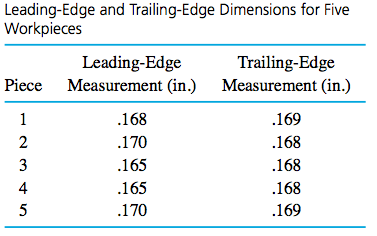
\includegraphics{../../fig/wooddata.png}
\end{center}
\begin{itemize}
\uncover<4->{\item Is the leading edge measurement different from the trailing edge measurement for a typical wood piece? Do a hypothesis test at $\alpha = 0.05$ to find out.}
\uncover<5->{\item Make a two-sided 95\% confidence interval for the true mean of the difference between the measurements.}
\end{itemize}
\end{frame}

\begin{frame}<handout:\answers>
\frametitle{Answers: wood product}
\begin{itemize}
\item Take paired differences (leading edge - trailing edge).
\end{itemize}
\begin{center}
\setkeys{Gin}{width=.7\textwidth} 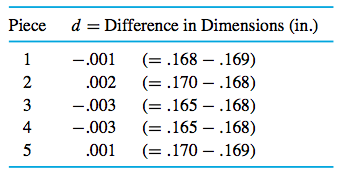
\includegraphics{../../fig/wooddiff.png}
\end{center}
\begin{itemize}
\pause \item The sample mean is $\ov{d} = -8 \times 10^{-4}$, and the sample standard deviation is $s_d = 0.0023$.
\pause \item Let $\mu_d$ be the true mean of the differences.
\end{itemize}
\end{frame}

\begin{frame}<handout:\answers>
\frametitle{Answers: wood product} \scriptsize
\begin{enumerate}[1. ]
\item $H_0: \mu_d = 0$, $H_a: \mu_d \ne 0$.
\pause \item $\alpha = 0.05$, $n = 5$.
\pause \item Since $\sigma_d$ is unknown, I use the test statistic:
\pause \begin{align*}
K = \frac{\ov{d} - 0}{s_d/\sqrt{n}}
\end{align*}
\begin{itemize}
\pause \item Assume $d_1, \ldots, d_5 \sim N(\mu_d, \sigma^2_d)$
\pause \item $K \sim t_{n -1} = t_4$.
\pause \item Reject $H_0$ if  $|K| > |t_{4, \ 1-\alpha/2}|$
\end{itemize}
\pause \item The moment of truth:
\begin{align*}
\uncover<9->{K} & \uncover<9->{=\frac{-8 \times 10^{-4} - 0}{0.0023/\sqrt{5}} =  -0.78} \\
\uncover<10->{t_{4, 1-\alpha/2}} & \uncover<10->{=t_{4, 1 - 0.05/2} = t_{4, 0.975} = 2.78}
\end{align*}
\uncover<11->{\item Since $|K| = 0.78 \not > 2.78 = t_{4, 0.975}$, I fail to reject $H_0$.}
\uncover<12->{\item There is not enough evidence to conclude that the leading edge measurements differ significantly from the trailing edge measurements.}
\end{enumerate}
\end{frame}

\begin{frame}<handout:\answers>
\frametitle{Answers: wood product} \scriptsize
\begin{itemize}
\item I can make a two-sided 95\% confidence interval for $\mu_d$ in the usual way:
\begin{align*}
&\uncover<2->{\left (\ov{d} - t_{4, \ 1 - \alpha/2} \cdot \frac{s}{\sqrt{n}}, \ \ov{d} + t_{4, \ 1 - \alpha/2} \cdot \frac{s}{\sqrt{n}}\right)} \\
\uncover<3->{=}&\uncover<3->{ \left (-8 \times 10^{-4} - t_{4, 0.975} \cdot \frac{0.0023}{\sqrt{5}}, \ -8 \times 10^{-4} + t_{4, 0.975} \cdot \frac{0.0023}{\sqrt{5}} \right ) } \\
\uncover<4->{=}& \uncover<4->{\left (-8 \times 10^{-4} - 2.78 \cdot 0.0010, \ -8 \times 10^{-4} + 2.78 \cdot 0.0010 \right)} \\
\uncover<5->{=}& \uncover<5->{(-0.00358, 0.00198)}
\end{align*}
\uncover<6->{\item We are 95\% confident that the true mean difference between leading edge and trailing edge measurements is between -0.00358 in and 0.001298 in.}
\end{itemize}
\end{frame}










\section{Two-Sample Inference: Large Samples}

\begin{frame}
\frametitle{Two-sample inference}
\begin{itemize}
\item Comparing the means of two distinct populations without pairing up individual measurements.
\pause \item Examples:
\begin{itemize}
\item SAT scores of high school A vs. high school B.
\pause \item Severity of a disease in women vs. in men. 
\pause \item Heights of New Zealanders vs. heights of Ethiopians.
\pause \item Coefficients of friction after wear of sandpaper A vs. sandpaper B.
\end{itemize}
\pause \item Notation:
\begin{center}
\begin{tabular}{ccc}
Sample & 1 & 2 \\ \hline
Sample size & $n_1$ & $n_2$ \\ [1ex]
True mean & $\mu_1$ & $\mu_2$ \\ [1ex] 
Sample mean & $\ov{x}_1$ & $\ov{x}_2$ \\ [1ex]
True variance & $\sigma^2_1$ & $\sigma^2_2$ \\ [1ex]
Sample variance & $s^2_1$ & $s^2_2$ 
\end{tabular}
\end{center}

\end{itemize}
\end{frame}


\begin{frame}
\frametitle{$n_1 \ge 25$ and $n_2 \ge 25$, variances known} \scriptsize
\begin{itemize}
\item We want to test $H_0: \mu_1 - \mu_2 = \#$ with some alternative hypothesis
\pause \item If $\sigma^2_1$ and $\sigma_2^2$ are known, use the test statistic:
\pause \begin{align*}
K = \frac{(\ov{x}_1 - \ov{x}_2) - \#}{\sqrt{\frac{\sigma^2_1}{n_1} + \frac{\sigma^2_2}{n_2}}}
\end{align*}
which has a $N(0,1)$ distribution if:
\begin{itemize}
\pause \item $H_0$ is true.
\pause \item The sample 1 points are iid with mean $\mu_1$ and variance $\sigma^2_1$, and the sample 2 points are iid with mean $\mu_2$ and variance $\sigma^2_2$.
\end{itemize}
\pause \item The confidence intervals (2-sided, 1-sided upper, and 1-sided lower, respectively) for $\mu_1 - \mu_2$ are:
\begin{align*}
&\uncover<7->{\left ((\ov{x_1} - \ov{x}_2) - z_{1 - \alpha/2} \sqrt{\frac{\sigma^2_1}{n_1} + \frac{\sigma^2_2}{n_2}} , \ (\ov{x_1} - \ov{x}_2) + z_{1 - \alpha/2} \sqrt{\frac{\sigma^2_1}{n_1} + \frac{\sigma^2_2}{n_2}} \right )} \\
&\uncover<8->{\left (-\infty , \ (\ov{x_1} - \ov{x}_2) + z_{1 - \alpha} \sqrt{\frac{\sigma^2_1}{n_1} + \frac{\sigma^2_2}{n_2}} \right )} \\
&\uncover<9->{\left ((\ov{x_1} - \ov{x}_2) - z_{1 - \alpha} \sqrt{\frac{\sigma^2_1}{n_1} + \frac{\sigma^2_2}{n_2}}, \ \infty \right )} 
\end{align*}
\end{itemize}
\end{frame}


\begin{frame}
\frametitle{$n_1 \ge 25$ and $n_2 \ge 25$, variances UNknown} \scriptsize
\begin{itemize}
\item If $\sigma^2_1$ and $\sigma_2^2$ are UNknown, use the test statistic:
\pause \begin{align*}
K = \frac{(\ov{x}_1 - \ov{x}_2) - \#}{\sqrt{\frac{s^2_1}{n_1} + \frac{s^2_2}{n_2}}}
\end{align*}
\pause \item And confidence intervals for $\mu_1 - \mu_2$:
\begin{align*}
&\uncover<4->{\left ((\ov{x_1} - \ov{x}_2) - z_{1 - \alpha/2} \sqrt{\frac{s^2_1}{n_1} + \frac{s^2_2}{n_2}} , \ (\ov{x_1} - \ov{x}_2) + z_{1 - \alpha/2} \sqrt{\frac{s^2_1}{n_1} + \frac{s^2_2}{n_2}} \right )} \\
&\uncover<5->{\left (-\infty , \ (\ov{x_1} - \ov{x}_2) + z_{1 - \alpha} \sqrt{\frac{s^2_1}{n_1} + \frac{s^2_2}{n_2}} \right )} \\
&\uncover<6->{\left ((\ov{x_1} - \ov{x}_2) - z_{1 - \alpha} \sqrt{\frac{s^2_1}{n_1} + \frac{s^2_2}{n_2}}, \ \infty \right )}
\end{align*}
\end{itemize}
\end{frame}

\begin{frame}
\frametitle{Example: packing weights}
\begin{itemize}
\item A company research effort involved finding a workable geometry for molded pieces of a solid. 
\pause \item One comparison made was between the weight (in grams) of molded pieces of a particular geometry that could be poured into a standard container, and the weight of irregularly shaped pieces (obtained through crushing), that could be poured into the same container. 
\pause \item $n_1 = 24$ crushed pieces and $n_2 = 24$ molded pieces were made and weighed.
\pause \item $\mu_1$ is the true mean packing weight of the crushed pieces, and $\mu_2$ is the true mean packing weight of the molded pieces.
\pause \item I want to formally test the claim that the crushed weights are greater than the molded weights.
\end{itemize}
\end{frame}

\newcounter{saveenum}
\begin{frame}
\frametitle{Example: packing weights}
\begin{enumerate}[1. ]
\item $H_0:  \mu_1 - \mu_2 = 0$, $H_a: \mu_1 - \mu_2 > 0$.
\pause \item $\alpha = 0.05$
\pause \item The test statistic is:
\pause \begin{align*}
K = \frac{(\ov{x}_1 - \ov{x}_2) - 0}{\sqrt{\frac{s^2_1}{n_1} + \frac{s^2_2}{n_2}}}
\end{align*}
\begin{itemize}
\pause \item $n_1$ and $n_2$ are each $< 25$, but each sample is normally distributed enough to flex that rule and allow $n_1 = n_2 = 24$.
\pause \item Assume the crushed weights are iid $(\mu_1, \sigma^2_1)$.
\pause \item Assume the molded weights are iid  $(\mu_2, \sigma^2_2)$.
\pause \item $K \sim N(0,1)$ under the null hypothesis.
\end{itemize}
\setcounter{saveenum}{\value{enumi}}

\end{enumerate}
\end{frame}

\begin{frame}
\frametitle{Example: packing weights}
\begin{enumerate}[1. ]
 \setcounter{enumi}{\value{saveenum}}
\item The moment of truth:
\begin{align*}
\uncover<2->{K} &\uncover<2->{=  \frac{(\ov{x}_1 - \ov{x}_2) - 0}{\frac{s^2_1}{n_1} + \frac{s^2_2}{n_2}}} \uncover<3->{= \frac{179.55 - 132.97 - 0}{\sqrt{\frac{(8.34)^2}{24} + \frac{(9.31)^2}{24}}}} \uncover<4->{= 18.3} \\
\uncover<5->{\text{p-value}} &\uncover<5->{= P(Z > K)} \uncover<6->{ = 1 - \Phi(K)} \uncover<7->{= 1 - \Phi(18.3)} \\
&\uncover<8->{= 4 \times 10^{-75}}
\end{align*}
\uncover<9->{\item With a p-value of $4 \times 10^{-75} < \alpha$, we reject $H_0$ in favor of $H_a$.}
\uncover<10->{\item There is overwhelming evidence that more crushed solid material by weight can be poured into the container than molded solid material.}
\end{enumerate}
\end{frame}

\begin{frame}
\frametitle{Example: packing weights}
\begin{itemize}
\item The analogous lower 95\% confidence interval for $\mu_1 - \mu_2$ is:
\begin{align*}
&\uncover<2->{\left ((\ov{x_1} - \ov{x}_2) - z_{1 - \alpha} \sqrt{\frac{s^2_1}{n_1} + \frac{s^2_2}{n_2}}, \ \infty \right )}  \\
&\uncover<3->{= \left ((179.55 - 132.97) - z_{0.95} \sqrt{\frac{(8.34)^2}{24} + \frac{(9.31)^2}{24}}, \ \infty \right )} \\
&\uncover<4->{= (46.58 - 1.64 \cdot 2.55, \ \infty)} \\
&\uncover<5->{= (42.40, \ \infty)}
\end{align*}
\uncover<6->{\item We're 95\% confident that the true mean packing weight of crushed solids is at least 42.40 g greater than that of the molded solids.}
\end{itemize}
\end{frame}


\begin{frame}
\frametitle{Example: packing weights}
\begin{center}
\setkeys{Gin}{width=.7\textwidth} 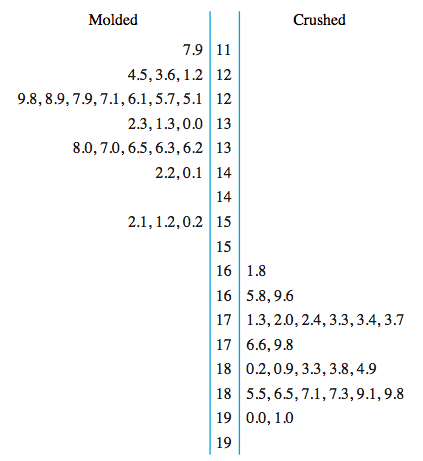
\includegraphics{../../fig/solidsstem.png}
\end{center}
\end{frame}


\begin{frame}
\frametitle{Your turn: anchor bolts} \scriptsize
\begin{itemize}
\item An experiment carried out to study various characteristics of anchor bolts resulted in 78 observations on shear strength (kip) of 3/8-in. diameter bolts and 88 observations on strength of 1/2-in. diameter bolts.
\end{itemize}
\begin{center}
\setkeys{Gin}{width=1\textwidth} 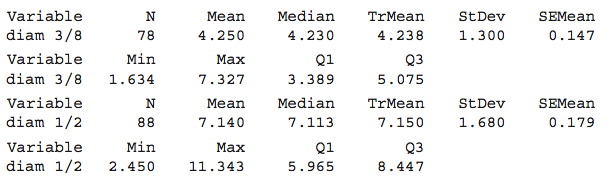
\includegraphics{../../fig/anchorboltsminitab.png}
\end{center}
\begin{itemize}
\pause \item Let Sample 1 be the 1/2 in diameter bolts and Sample 2 be the 3/8 in diameter bolts.
\pause \item Using a significance level of $\alpha = 0.01$, find out if the 1/2 in bolts are more than 2 kip stronger (in shear strength) than the 3/8 in bolts. 
\pause \item Calculate and interpret the appropriate 99\% confidence interval to support the analysis.
\end{itemize}
\end{frame}


\begin{frame}<handout:\answers>
\frametitle{Answers: anchor bolts}
\begin{itemize}
\item $n_1 = 88, \ n_2 = 78$.
\pause \item $\ov{x}_1 = 7.14$, $\ov{x}_2 = 4.25$ 
\pause \item $s_1 = 1.68$, $s_2 = 1.3$
\end{itemize}
\begin{enumerate}[1. ]
\pause \item $H_0: \mu_1 - \mu_2 = 2$, $H_a: \mu_1 - \mu_2 > 2$
\pause \item $\alpha = 0.01$
\pause \item The test statistic is:
\pause \begin{align*}
K = \frac{(\ov{x}_1 - \ov{x}_2) - 2}{\sqrt{\frac{s^2_1}{n_1} + \frac{s^2_2}{n_2}}}
\end{align*}
\begin{itemize}
\pause \item Assume:
\begin{itemize}
\pause \item $H_0$ is true.
\pause \item Sample 1 points are drawn from iid $(\mu_1, \sigma^2_1)$ distributions.
\pause \item Sample 2 points are drawn from iid $(\mu_2, \sigma^2_2)$ distributions.
\end{itemize}
\pause \item Then, $K \sim N(0,1)$
\end{itemize}
\end{enumerate}
\end{frame}

\begin{frame}<handout:\answers>
\frametitle{Answers: anchor bolts}
\begin{enumerate}[1. ]
 \setcounter{enumi}{\value{saveenum}}
\item The moment of truth:
\begin{align*}
\uncover<2->{K} &\uncover<2->{=  \frac{(\ov{x}_1 - \ov{x}_2) - 2)}{\frac{s^2_1}{n_1} + \frac{s^2_2}{n_2}}} \uncover<3->{ = \frac{(7.14 - 4.25) - 2}{\sqrt{\frac{(1.68)^2}{88} + \frac{(1.3)^2}{78} }}}\uncover<4->{ = 3.84} \\
\uncover<5->{\text{p-value}} &\uncover<5->{= P(Z > K) } \uncover<6->{= 1 - P(Z \le K) = 1 - P(Z \le 3.84)}  \\
&\uncover<7->{= 1 - \Phi(3.84) \approx 0}
\end{align*}
\uncover<8->{\item With a p-value $\approx 0 < \alpha = 0.01$, we reject $H_0$ in favor of $H_a$.}
\uncover<9->{\item There is overwhelming evidence that the 1/2 in anchor bolts are more than 2 kip stronger in shear strength than the 3/8 in bolts.}
\end{enumerate}
\end{frame}



\begin{frame}<handout:\answers>
\frametitle{Answers: anchor bolts}
\begin{itemize}
\item I use a lower confidence interval for $\mu_1 - \mu_2$:
\end{itemize}
\begin{align*}
&\uncover<2->{\left ((\ov{x_1} - \ov{x}_2) - z_{1 - \alpha} \sqrt{\frac{s^2_1}{n_1} + \frac{s^2_2}{n_2}}, \ \infty \right )}  \\
&\uncover<3->{= \left ((7.14 - 4.25) - z_{0.99} \cdot \sqrt{\frac{1.68^2}{88} + \frac{1.3^2}{78}}, \ \infty \right )} \\ 
&\uncover<4->{= (2.89 - 2.33 \cdot 0.232, \ \infty )} \\
&\uncover<5->{= (2.35, \ \infty)}
\end{align*}
\begin{itemize}
\uncover<6->{\item We're 99\% confident that the true mean shear strength of the 1/2 in anchor bolts is at least 2.35 kip more than the true mean shear strength of the 3/8 in anchor bolts.}
\end{itemize}
\end{frame}









\end{document}
